%!TEX encoding = IsoLatin
\documentclass[conference]{IEEEtran}

\usepackage{cite}
\usepackage{graphicx}
\usepackage{amsmath}
\usepackage{algorithmic}
\usepackage{fixltx2e}
\usepackage{stfloats}
\usepackage{url}
\usepackage{hyperref}
\usepackage[latin1]{inputenc}
\usepackage{lipsum}
\usepackage{coolmath}
\usepackage[hang,small]{caption}
\graphicspath{{Images/}}

\title{Relevance Vector Machine and Sparse Vector Regression : a study on the sparsity versus performance tradeoff}
\author{
	\IEEEauthorblockN{Hadrien Hendrikx}
	\IEEEauthorblockA{
					School of Computer and Communication Sciences (IC)\\
					\'Ecole Polytechnique \\ F�d�rale de Lausanne\\
					Lausanne, Switzerland\\
					hadrien.hendrix@epfl.ch
					}\\
	\and
	\IEEEauthorblockN{Gregoire Gallois-Montbrun}
	\IEEEauthorblockA{
					School of Engineering (STI)\\
					\'Ecole Polytechnique \\ F�d�rale de Lausanne\\
					Lausanne, Switzerland\\
					gregoire.gallois-montbrun@epfl.ch
					}
	\and
	\IEEEauthorblockN{Louis Faury}
	\IEEEauthorblockA{
					School of Engineering (STI)\\
					\'Ecole Polytechnique \\ F�d�rale de Lausanne\\
					Lausanne, Switzerland\\
					louis.faury@epfl.ch
					}
	}
	
\begin{document}

	\maketitle
	
	\begin{abstract}
		Over the last decade, sparse kernel machines have been at the center of a general interest from both the research community and the industrial one. Once trained, their inherent sparsity allows for fast computations, even on large datasets. 
		\newline This report, written in the context of a machine learning coding project, compares two sparse regression techniques. \newline After introducing some theoretical aspects on Support Vector Regression (SVR) and the Relevance Vector Regression (RVR), we introduce two datasets (an artificial one well as a real one) that we will use as baselines for experimental comparisons between the two methods. 
		\newline We will then focus the comparison on a few key features. Namely, we will analyze the tradeoff found between generalization and sparsity in the two methods. Other issues such as robustness (behavior far from data, dataset scavenging and data chunking) and complexity will also be tackled. 
	\end{abstract}
	
	\section{Introduction}
	{
		We hereinafter focus on regression tasks : from a dataset $\{X,\mathbf{t}\} \in\mathbb{R}^{N,d}\times\mathbb{R}^N$, we wish to learn a function $f$ such that $f(X)\simeq \mathbf{t}$. 
		\newline The simplest method to perform such a task is to consider that $f(\cdot)$ is a linear function of a non-linear mapping of the input $x$, corrupted by a normally distributed noise of precision  $\beta$ 
		\begin{equation}
			t = w^T\phi(x) + \eta, \quad \eta \sim \normalDb{\eta}{0}{\beta^{-1}} 
		\end{equation} 
		with $\phi\, : \, \mathbb{R}^d \to \mathbb{R}^m$ a non-linear transformation. 
		Therefore, $p(t\, \vert \, w,\beta)\sim \normalDb{t}{w^T\phi(x)}{\beta^{-1}}$ and the \emph{maximum-likelihood} solution is given by the minimizer of the opposite of the log-likelihood : 
		\begin{equation}
			w_{MLE} = \argmin{w}{\frac{1}{2}\sum_{n=1}^N\left\{w^T\phi(x_n) - t_n\right\}^2}
		\end{equation}
		To avoid overfitting, a regularizer term is often added to the cost function :
			\begin{equation} 
							E(w) = \frac{1}{2}\sum_{n=1}^N\left\{w^T\phi(x_n) - t_n\right\}^2 + \frac{\lambda}{2}\lVert w \rVert ^2
							\label{eq::ridge}
			\end{equation}
		even if some more advanced methods (Bayesian learning for instance) can also be used to avoid prevent data overfit. 
	}
	\section{Theoretical background}
	{
		\subsection{Support Vector machine for Regression}
		{
			The Support Vector machine for Regression (SVR) extends the SVM method for regression tasks.
			\newline
			To obtain a sparse solution, the likelihood term in (\ref{eq::ridge}) is replaced by an $\eps$-\emph{insensitive error function} (see \cite{vapnik1995nature}) denoted $E_\eps(\cdot)$ with : 
			\begin{equation}
				\label{eq::loss}
				E_\eps(y(x)-t) = \left\{
								\begin{aligned}
								&0, \quad &\text{ if } \vert y(x)-t\vert < \eps\\
								& \vert y(x)-t\vert \quad &\text{otherwise}  
								\end{aligned}\right.
			\end{equation}
			Therefore, the quantity to be minimized can be expressed as : 
			\begin{equation}
				J(w) = \frac{C}{n}\sum_{n=1}^N E_\eps(w^T\phi(x_n)-t_n) + \frac{1}{2}\lVert w \rVert ^2
			\end{equation}
			where $C$ is a regularization parameter. 
			\newline 
			As for the SVM, one can introduce \emph{slack variables} in order to transform this optimization program into a Quadratic Programming (QP) problem (quadratic objective, linear constraints) : 
			
			\begin{mini}|s|[2]
  				 {w,b}{\frac{1}{2}\lVert w \rVert^2 + \frac{C}{n}\sum_{i=1}^n{\left(\xi_i + \hat{\xi}_i\right)}}
  				 {\label{eq::svr}}{}
   				\addConstraint{\xi, \hat{\xi}}{\geq 0}{\text{ (row wise) }}
  				 \addConstraint{w^T\phi(x_i)+b + \eps + \xi_i  }{\geq t_i,\quad}{i=1,\hdots,n}
				\addConstraint{w^T\phi(x_i)+b - \eps - \hat{\xi}_i  }{\leq t_i,\quad}{i=1,\hdots,n}
			\end{mini}
				
			Once the problem solved, predictions are made using : 
			\begin{equation}
				y(x) = \sum_{n=1}^N (a_n - \hat{a}_n)k(x,x_n) + b
			\end{equation}
			where we introduced the kernel function $k(x,x') = \phi(x)^T\phi(x')$. The coefficients $\{a_n\}$ and $\{\hat{a}_n\}$ actually are Lagrange multipliers for the QP problem (\ref{eq::svr}), and provide a \emph{sparse} solution  - only a few data points are used for regression. Those are called \emph{support vectors}, and are so that  $a_n \neq 0$ or $\hat{a}_n\neq 0$ - in other words, those that lie on the boundary or outside of the $\eps$-tube defined by the loss function in equation (\ref{eq::loss}). \newline
			As for the SVM, one can adopt a $\nu$-SVR formulation (see \cite{scholkopf2000new}) to have a \emph{lower-bound control} on the number of retained support vectors. 
		}
		\subsection{Relevance Vector machine for Regression}
		{
			The SVR therefore provides a useful tool for obtaining sparse regression machine. However, it suffers from a \emph{number of limitations}, such as an output representation as decision rather than posterior probability, the need to estimate hyper-parameters (kernel width, penalization parameter) via \emph{held-out methods} (like cross-validation), or the need for the kernel to be a Mercer kernel type (positive definite). 
			\newline
			The Relevance Vector Machine for regression is a \emph{Bayesian sparse kernel technique} that shares many of the SVR's characteristics while avoiding its limitations. It instantiates a model intended to mirror the structure of the SVR : 
			\begin{equation}
				y(x) = \sum_{n=1}^{N+1}w_nk(x,x_n)
			\end{equation}
			where the bias $b$ is included in the predictor $w$ and $k(\cdot,\cdot)$ is an arbitrary kernel (not necessarily positive definite). Assuming i.i.d data sample with Gaussian noise of precision $\beta$, the likelihood writes : 
			\begin{equation}\label{eq::rvr_likelihood}
				\condp{\mathbf{t}}{X,w,\beta} = \prod_{n=1}^N \normalDb{t_n}{y(x_n)}{\beta}
			\end{equation}
			The predictor $w$ is given a centered Gaussian prior distribution :
			\begin{equation}
				\condp{w}{\alpha} = \prod_{i=1}^{N+1} \normalDb{w_i}{0}{\alpha_i^{-1}}
			\end{equation}
			introducing a separate precision parameter $\alpha_i$ for each weight parameter $w_i$. 
			\newline 
			This leads to a Gaussian posterior distribution over $w$ : 
			\begin{equation}
				\begin{aligned}
					\condp{w}{\mathbf{t},X,\alpha,\beta} &= \condp{\mathbf{t}}{w,X,\beta}\condp{w}{\alpha}\\
												&= \normalDb{w}{m}{\Sigma}
				\end{aligned}
			\end{equation}
			where 
			\begin{equation}
				\begin{aligned}
					m &= \beta \Sigma \boldsymbol{\phi}^T t\\
					\Sigma &= \left(A+\beta \boldsymbol{\phi}^T\boldsymbol{\phi}\right)^{-1}, \qquad A = \text{diag}(\alpha_i)
				\end{aligned}
				\label{eq::posterior}
			\end{equation}
			In a full Bayesian approach, $\alpha$ and $\beta$ are both given prior distributions. However, this leads to intractable computations when computing predictions. The use of \emph{empirical Bayes} solves this problem, by approximating $\alpha$ and $\beta$ by their maximum-a-posteriori value (also known as the \emph{evidence approximation} or type-2 maximum likelihood). \newline
			As a result of approximation, a proportion of parameters $\alpha_i$ are driven to infinite values, constraining the corresponding weights $w_i$ to have $0$ mean and infinite precision, and hence are set to $0$. The resulting predictions are therefore sparse in data-points, and the inputs $\{x_n\}$ corresponding to non-zero weights are called \emph{relevance vectors}. Once the optimal values $\alpha^*$ and $\beta^*$ found, the predictive distribution over $y$ can therefore be computed using $\alpha^*$ and $\beta^*$. 
			\newline The sparsity analysis of the RVR leads to a practical algorithm for optimizing the hyper-parameters that has significant speed advantages, and is referred to as \emph{automatic relevance determination}. The full algorithm and its justification can be found in \cite{bishop2006pattern} and \cite{tipping2003relevance}.
			\newline Furthermore, the RVR provides a posterior distribution over the predictor, leading to the following \emph{predictive distribution} (unlike the SVR which only provide a posterior decision) : 
			\begin{equation}
				\begin{aligned}
					\condp{t}{x,X,\mathbf{t},\alpha,\beta} &= \int_w \condp{t}{w,x,\beta}\condp{w}{X,\mathbf{t},\alpha}dw\\
					&= \normalDb{t}{m^T\phi(x)}{\beta^{-1}+\phi(x)^T\Sigma \phi(x)}
				\end{aligned}
				\label{eq::predictive}
			\end{equation}
			with $m$ and $\Sigma$ the first moments of the posterior (see (\ref{eq::posterior}))
		}
		\subsection{Theoretical method comparaison}
		{
			\subsubsection{Complexity}
			{
				When comparing the SVR's and the RVR's complexity, one must distinguish complexity at training time and at testing time. \newline
				Training the SVR sums up in solving a large quadratic-programing (QP) problem. A popular approach to do that implies breaking up the initial QP into smaller problems, solvable analytically, and is called \emph{Sequential Minimization Optimization} (SMO). It requires a linear (with respect to the datapoints) amount of memory, and scales between linear and quadratic complexity in the training set size (see \cite{platt1998sequential}). At test time, the complexity is linear in the number of support vectors. \newline
				Training a RVM involves optimizing a non-convex function. For a model with $M$ basis functions, the RVM requires the inversion of a $M\times M$ matrix, which requires from $O(M^{2.7})$ to $O(M^{3})$, which is as we just saw larger than the SVR's cost. However, parameters are determined automatically and in one run when training a RVR, while the hyper-parameters typically need several runs (f-fold cross-validation) to be estimated. At testing time, the RVR's complexity grows linearly with the number of relevance vectors.  
			}
			\subsubsection{Performance}
			{
				We just named one of the major pros of using RVR - there is no need for using held-out methods to estimate hyper-parameters, as they are automatically determined through automatic relevance detection (expect for parametric basis functions). Also, it has been shown \cite{platt1998sequential, bishop2006pattern} that RVR leads to \emph{sparser solutions, without loss of generalization abilities} (on the contrary, the RVR usually performs better than the SVR). We will try to observe this in the experiments derived hereinafter.
			}
		}
	}
	\section{Experimental results}
	{
		\subsection{Datasets presentation}
		{
			\subsubsection{Artificial dataset}
			{
				The goal of using an artificial dataset is to be able to produce visual outputs to evaluate the performance of the two methods on a simple regression problem, hence the need to work in a one dimensional dataset. 
				\newline The dataset was generated from the $sinc(\cdot)$ function, on the interval $[-5,5]$. Points were randomly sampled from this interval, applied the $sinc$ function and added a Gaussian distributed centered noise of variance $\sigma^2 = 0.01$. 
				\newline The following table sums up the dataset characteristics. 
				\vspace{3pt}
				
				\noindent\begin{tabular}{|c|c|c|c|c|}
				\hline 
					\textbf{Dimension} & \textbf{Points} & \textbf{Support} & \textbf{Noise variance} & \textbf{Outlier} \\
					\hline
					1 & 100 & [-5,5] & 0.01 & No\\
					\hline
				\end{tabular}
				
				\begin{figure}[h!]
					\centering
					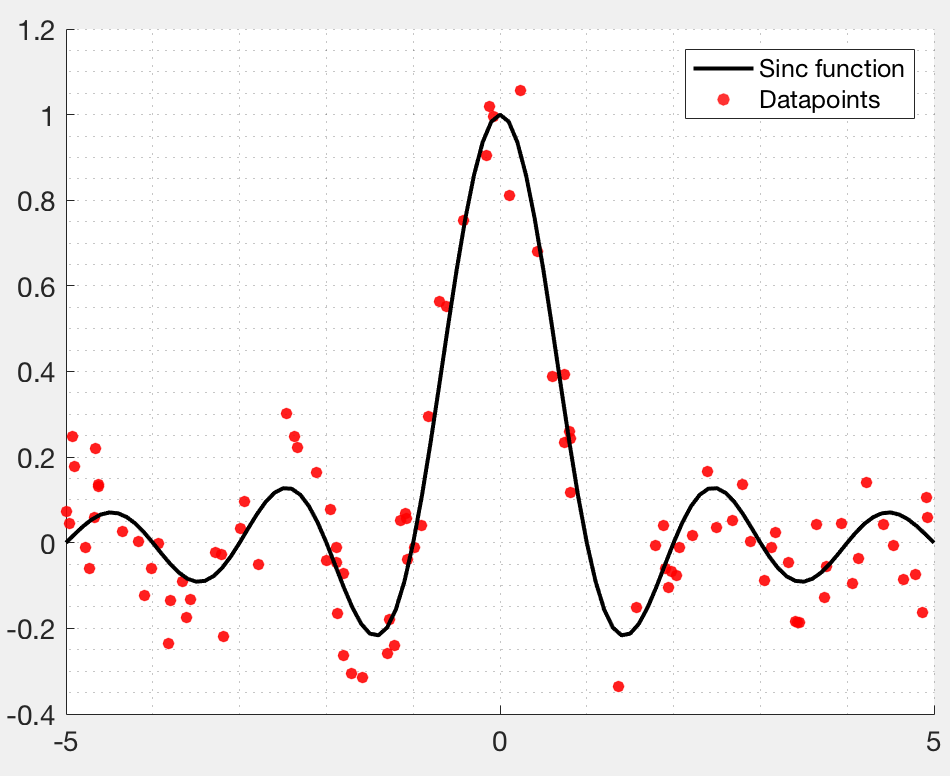
\includegraphics[width=0.6\linewidth]{dataset_1d}
					\caption{The 1D artificial dataset}
				\end{figure}
			}
			\vspace{5pt}
			
			\subsubsection{Real dataset}
			{
				%This dataset, known as the Online News Popularity dataset, provide informations about a web article (number of words, number of link to other articles, number of images or videos, ..) to predict its number of shares in social network (see \cite{fernandes2015proactive} for full details). The following table sums up the dataset characteristics. 
				
			        %\begin{center}
				%\noindent\begin{tabular}{|c|c|}
				%	\hline 
				%	\textbf{Dimension} & \textbf{Points} \\
				%	\hline
				%	58 & 30493\\
				%	\hline
				%\end{tabular}
				%\end{center}
				This dataset, known as the Airfoils Self-Noise dataset provides informations about design of various airfoils and physical environment (free stream velocity, angle of attack, chord length, frequency, suction side thickness) in order to predict the resulting sound pressure level in dB (see \cite{brooks1989} for full details). The following table sums up the dataset characteristics. All experiments were performed after standardization of the dataset.
				
				\vspace{3pt}
				
				\begin{center}
				\noindent\begin{tabular}{|c|c|}
					\hline 
					\textbf{Dimension} & \textbf{Points} \\
					\hline
					5 & 1503\\
					\hline
				\end{tabular}
				\end{center}	
			}
		}
		\subsection{Implementation}
		{
			We hereinafter describe different computations and results obtained on the artificial data with both the SVR and the RVR. Discussion on the two methods advantages and drawbacks will be held in the next section.
			
			\subsubsection{Support Vector Regression}
			{
				We implemented both the $\eps$-SVR and the $\nu$-SVR on the artificial dataset. We used the \texttt{libsvm} library (see \cite{libsvm}) with a radial-basis function kernel : 
				\begin{equation}
					\forall x,x', \quad k(x,x') = \exp{\left( -\frac{\lVert x -x'\rVert^2}{\sigma^2}\right)}
				\end{equation}
				
				We therefore tuned three hyper-parameters : $\sigma$ (kernel width), $C$ (penalization factor) and $\nu$ (resp. $\eps$) for the $\nu$-SVR (resp. $\eps$-SVR). Figures (\ref{epsSVR}) and (\ref{nuSVR}) display the regressive function obtained for three given parameters for both methods on the artificial dataset. For the $\nu$-SVR, the corresponding $\eps$-insensitive tube was computed thanks to the values of the final Lagrange multipliers (a Lagrange multiplier strictly inferior to $C$ indicates a point laying on the $\eps$-tube). 
				\begin{figure}
					\begin{center}
						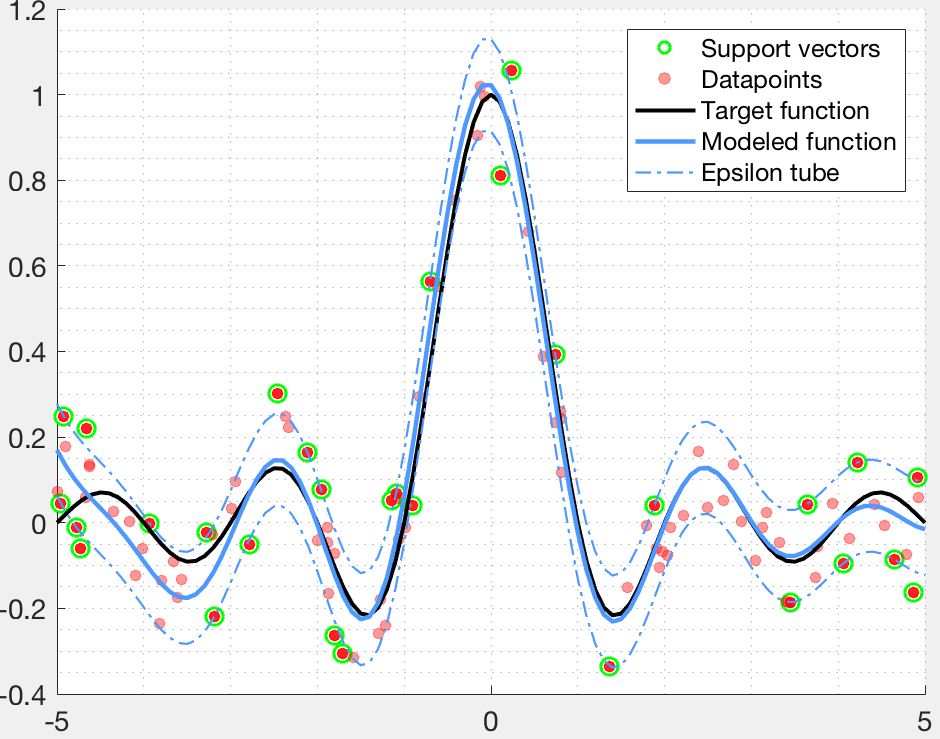
\includegraphics[width=0.85\linewidth]{nuSVR_nu02_C100_width02}
						\caption{$\nu$-SVR with : $C=100$, $\nu=0.2$, $\sigma = 1.5$}
						\label{nuSVR}
					\end{center}
				\end{figure}
				\begin{figure}				
					\begin{center}
						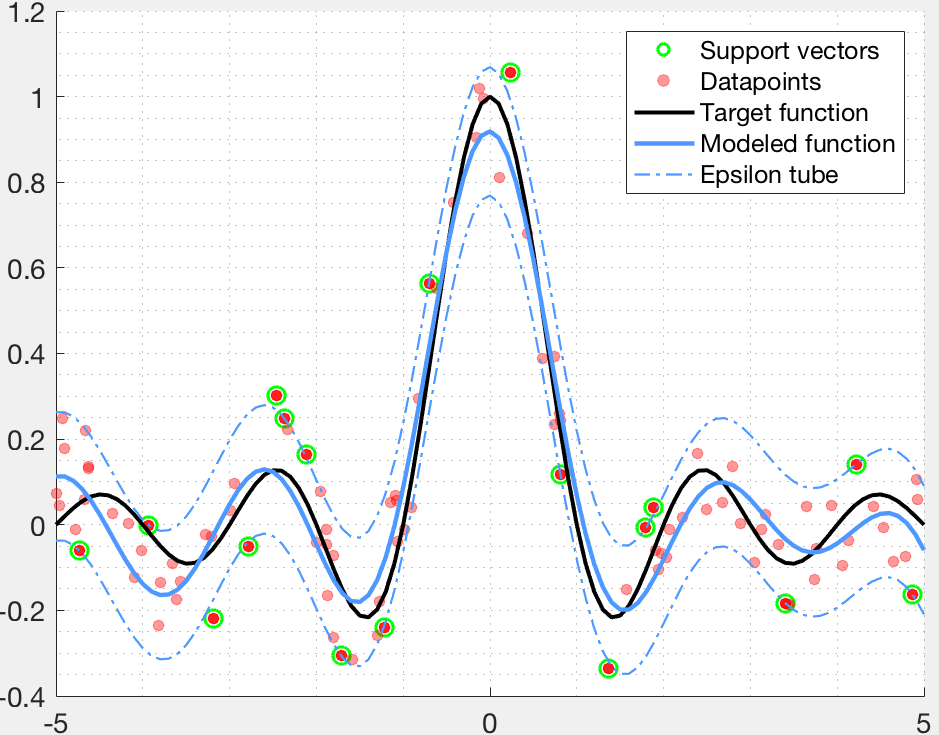
\includegraphics[width=0.85\linewidth]{epsSVR_eps015_C50_width2}
						\caption{$\eps$-SVR with : $C=50$, $\eps=0.15$, $\sigma = 2$}
						\label{epsSVR}
					\end{center}
				\end{figure}
			}
			\subsubsection{Relevance Vector Regression}
			{
				A similar work was conducted with the RVR, by using the \texttt{SparseBayes} library written by Mike Tipping. The same kernel (RBF) was used. Therefore, the only hyper-parameter to be fixed is the kernel's width $\sigma$ (since automatic relevance detection automatically finds the best $\beta$ and $\alpha$). For regression, we plot the mean of the \emph{predictive distribution} as well as it's standard deviation (see (\ref{eq::predictive})).
				
				\begin{figure}
					\begin{center}
						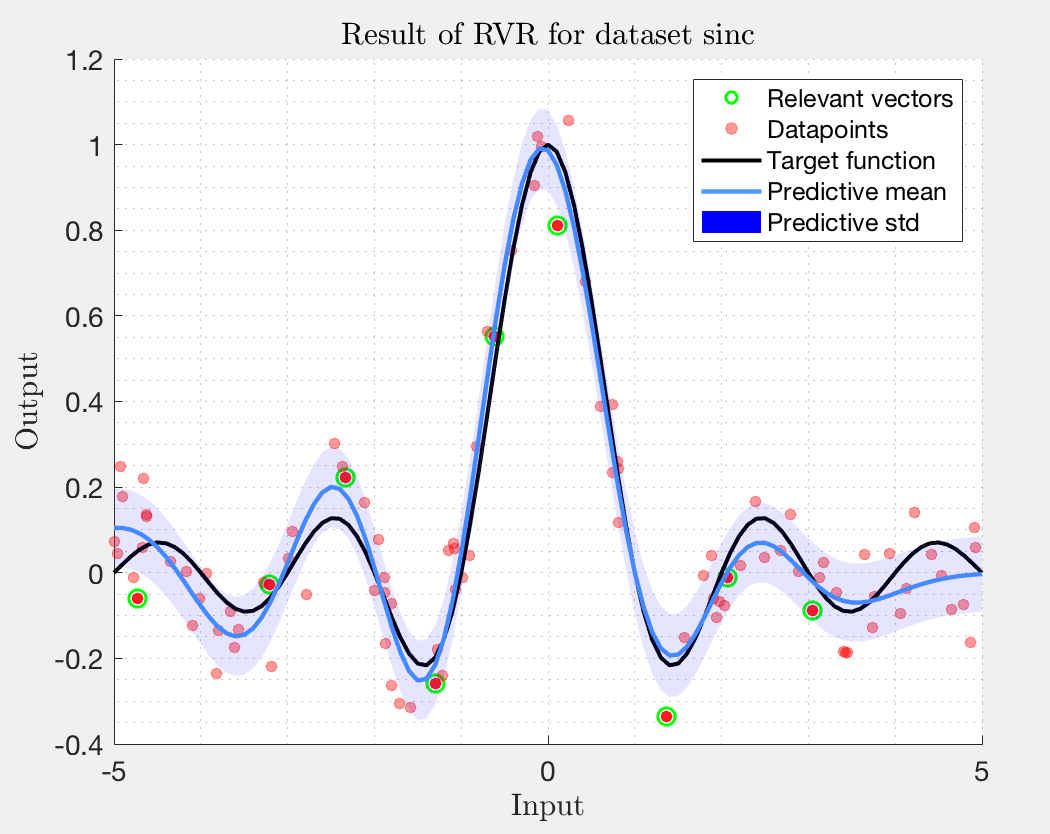
\includegraphics[width=0.85\linewidth]{RVR_width1}
						\caption{RVR with : $\sigma = 1$}
						\label{nuSVR}
					\end{center}
				\end{figure}
			}
		
		}
		\subsection{Cross-validation}
		{
			\subsubsection{A sparse regression evaluative metric}
			{
			To infer the best hyper-parameters for all three algorithms ($\epsilon$-SVR, $\nu$-SVR and RVR), grid-search cross-validation is used. The metric we used to evaluate performance of the algorithms is derived from the BIC (Bayesian Information Criterion, see \cite{bishop2006pattern}). Among the properties of this metric is the ability to evaluate a compromise between complexity and likelihood of different models. We want to reproduce this characteristic to evaluate the performance versus sparsity tradeoff found by different models. The following lines intent to motivate the metric we chose to use. 
			\newline
			The general formula of the BIC metric  is:
			\begin{equation}
				BIC = -2ln(L) + kln(N)
			\end{equation}
			where $L$ corresponds to the likelihood of the model, $k$ is the number of parameters of the model and $N$ is the number of data-points. In the particular case we wish to tackle (\textit{i.e} measuring a trade-off between regression performance and sparsity), the BIC appears to be a reasonable metric, although some adjustments are needed to adapt it to a regression task. 
			Assuming independent, normally distributed noise, the likelihood can naturally be related to the Mean Square Error (MSE) :
			\begin{equation}
				ln(L) = -\frac{N}{2\sigma^2}MSE
			\end{equation}
			 where $\sigma^2$ corresponds to the variance of the dataset's noise.
			 \newline For both algorithms, the number of parameters $k$ is directly proportional to the number of relevant vectors (respectively support vectors). Therefore a reasonable metric to measure the goodness of a sparse regression model would be 
			\begin{equation}
				BICSR =  N\frac{MSE}{\sigma^2} + N_{SV}ln(N)
			\end{equation}
			where ${N_{SV}}$ is the number of relevance (or support) vectors, and $BICSR$ holds for Bayesian Information Criterion for Sparse Regression. Minimizing this metric indeed implies minimizing the MSE while linearly penalizing the number of support vectors. Some other kind of penalization (quadratic, exponential) could also be used. The discussion of the choice of this penalization, as well as the validation of the well behavior of this metric is held in (\ref{section::discussion}). 
			
			We wish to emphasize the fact that this metric is not the commonly used BIC metric, but rather an adaptation of it to sparse regression (and therefore a measure of trade-off between performance (MSE) and sparsity).
			}
			\subsubsection{Grid-search cross-validation}
			{
				In the following, we performed 50-fold cross-validation with a 0.75 training-test ratio, using the $BICSR$ previously defined.
				 
				\begin{figure}
					\begin{center}
						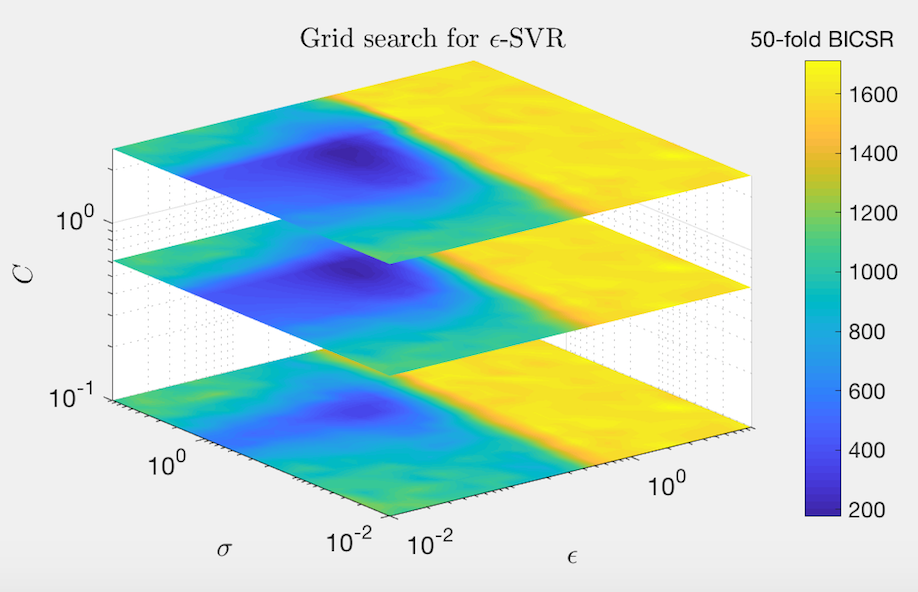
\includegraphics[width=0.85\linewidth]{gridSearch_epsSVR_BIC_sinc}
						\caption{Grid search for $\epsilon$-SVR over $\epsilon$, $C$ and $\sigma$ for sinc dataset \\ Best hyperparameters: $\epsilon = 0.17$, $C = 2.40$, $\sigma = 1.17$}
						\label{fig::gridSearch_epsSVR_sinc}
					\end{center}
				\end{figure}
				
				\begin{figure}
					\begin{center}
						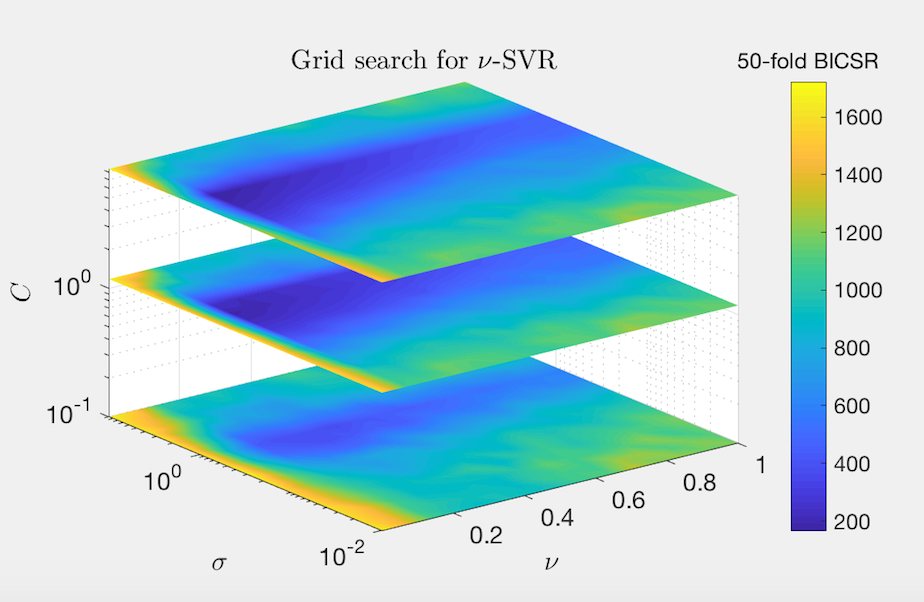
\includegraphics[width=0.85\linewidth]{gridSearch_nuSVR_BIC}
						\caption{Grid search for $\nu$-SVR over $\nu$, $C$ and $\sigma$ for sinc dataset \\ Best hyperparameters: $\nu = 0.057$, $C = 1.52$, $\sigma = 1.13$}
						\label{fig::gridSearch_nuSVR_sinc}
					\end{center}
				\end{figure}
			
			There are three hyperparameters to estimate for $\epsilon$-SVR. $\epsilon$ represents the width of the insensitive tube, and its optimal value should be close to the actual value for standard deviation of the output noise. The explored range [0.001, 10] seemed therefore adequate. $C$ penalizes for distances between points lying outside the $\epsilon$-tube and the border of the tube, it is hard to estimate beforehand the amount of order of the optimal value so that grid search was performed on the interval [0.1, 1000]. Finally, the kernel width $\sigma$ represents the region of influence of the different support vectors. Given the spacing of inputs for the dataset, a good value should lie near 1 so that explored range was set to [0.001, 10].
			\newline For $\nu$-SVR, $\nu$ necessarily lies in the interval ]0,1[, the explored range, and represents a lower bound on the fraction of support vectors. Other considerations for kernel width $\sigma$ and penalization factor $C$ still hold.
			
			Figures (\ref{fig::gridSearch_epsSVR_sinc}) and (\ref{fig::gridSearch_nuSVR_sinc}) display grid search results for both $\epsilon$-SVR and $\nu$-SVR in the form of heat-maps. If we fix $C$, we can distinctively see that the objective function forms a well. Changing the value of $C$ only changes the size of the well and its value but not the global behaviour, which suggests that this parameter has little influence on the result as long as values are not too far from the optimal. This leads us to believe that there is a global minimum for our objective function, that this minimum is captured by our grid and therefore that the result of our grid search is reliable. The form of the regions is slightly different between $\epsilon$-SVR and $\nu$-SVR but the general behaviour are the same. 
			
			For $\epsilon$-SVR, the plateau corresponding to highest values of $\epsilon$ corresponds to models where all points lie inside the $\epsilon$-tube. Finally, as expected, optimal models for both methods are very close, since they share most of their support vectors, therefore showing the equivalence between both approaches. Both lead to a total of 14 support vectors, corresponding to a Mean square error of 0.013.
			
			 %As expected both selected models are almost the same therefore showing the equivalence between both approaches. Both lead to a total of 14 support vectors.

			
				%		Figures (\ref{fig::gridSearch_epsSVR_sinc}) and (\ref{fig::gridSearch_nuSVR_sinc}) display grid search results for both $\epsilon$-SVR and $\nu$-SVR in the form of heat-maps.  We can distinctively notice wells for both methods. It demonstrates the existence of parameters combinations that minimize our $BICSR$ metric. 
			
				\begin{figure}
					\begin{center}
						\includegraphics[width=0.75\linewidth]{gridsearch_RVR}
						\caption{Grid search for $RVR$  over $\sigma$ for sinc dataset. Best hyperparameter: $\sigma = 1.28$}
						\label{fig::gridSearch_RVR_sinc}
					\end{center}
				\end{figure}
			\noindent Figure (\ref{fig::gridSearch_RVR_sinc}) displays grid-search results for the RVR over kernel width $\sigma$, the only hyperparameter for this method. Found optimal value $1.28$ again confirms expectations that the order of magnitude is well chosen since it is close to the value chosen for SVR methods. Corresponding number of relevant vectors is eight, leading to a MSE of 0.01. As a result, for this particular metric which demonstrates good properties concerning the sparsity/accuracy trade-off, as will be demonstrated in section (\ref{section::discussion}), the RVR optimal model leads to a sparser and more accurate solution than optimal SVR models.
			
			% TODO : some more commenting over the different figures (presence of a well and plateau, .. )
			% TODO : motivate bounds
			% TODO : use the following rather in the discussion part 
%			The $BIC$ criterion is a way to take model complexity into account when choosing an appropriate model. In our setting, the complexity is governed by the number of support vectors used and we are interested in the relationship between sparsity (the more support vectors the more complex the function can be) and performance (measured by the $MSE$). We analyze this tradeoff in figure \ref{fig::ROC_sinc} for the $sinc$ dataset. We can see that in terms of pure $MSE$ minimization both $\nu-SVR$ and $C-SVR$ perform slightly better than $RVR$ but at a very high cost in terms of sparsity since they have respectively $3$ and almost $5$ times more support vectors. For the hyperparameters that minimize the $BIC$ criterion, $SVR$ achieves a sparsity that is comparable to that of $RVR$ (although still there are still more support vectors) but this comes at the cost of a sharp rise of the $MSE$ of around $10\%$ for the $\nu-SVR$ and almost $50\%$ for the $C-SVR$. We can conclude that $RVR$ should be prefered as soon as the sparsity of the model is a concern.
			}
							
			\subsection{Real dataset}
			{
				\noindent For this dataset, no prior knowledge on the variance of the noise affecting the outputs was available. As a consequence, it had to be estimated before applying $BICSR$ metric to the dataset (see section (\ref{section::discussion})). As we have seen in the previous study, Relevance Vectors Regression always provides sparse solutions while estimating output noise via parameter $\beta$. To find a relevant value for kernel width, a first grid search was therefore performed for RVR with MSE. Corresponding estimation for $\beta$ (equals to 2.4) was then used to evaluate $BICSR$ for all models.  				
				We then performed grid search using 10-fold cross validation to estimate best values for algorithms hyperparameters. Due to higher dimensionality and to an higher number of points, training test ratio was decreased to 0.5.
				
								
				\begin{figure}
					\begin{center}
						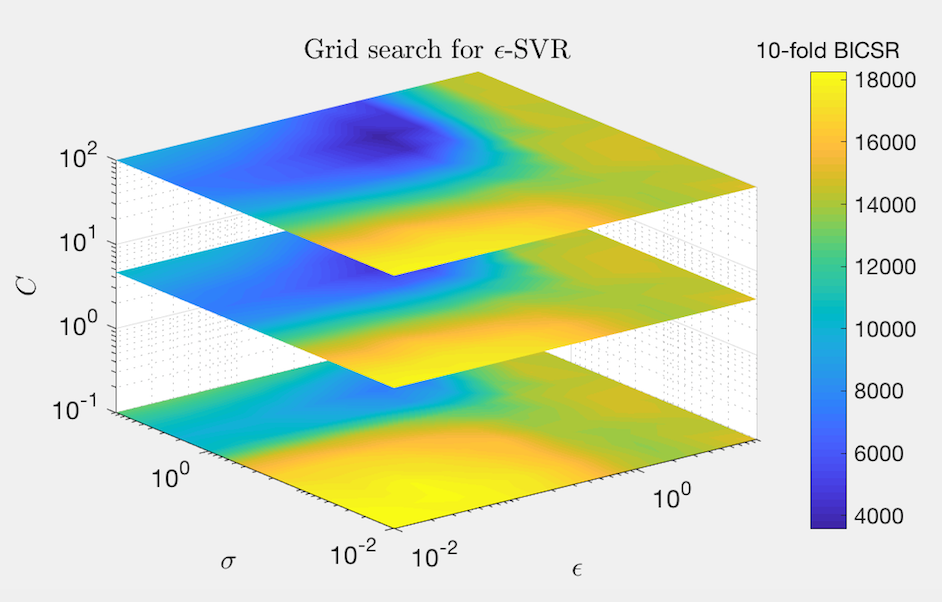
\includegraphics[width=0.85\linewidth]{gridSearch_epsSVR_BIC_airfoils}
						\caption{Grid search for $\epsilon$-SVR over $\epsilon$, $C$ and $\sigma$ for airfoils dataset \\ Best hyperparameters: $\epsilon = 0.46$, $C = 100$, $\sigma = 2.15$}
						\label{fig::gridSearch_BIC_epsSVR_airfoils}
					\end{center}
				\end{figure}
				
				
								
				\begin{figure}
					\begin{center}
						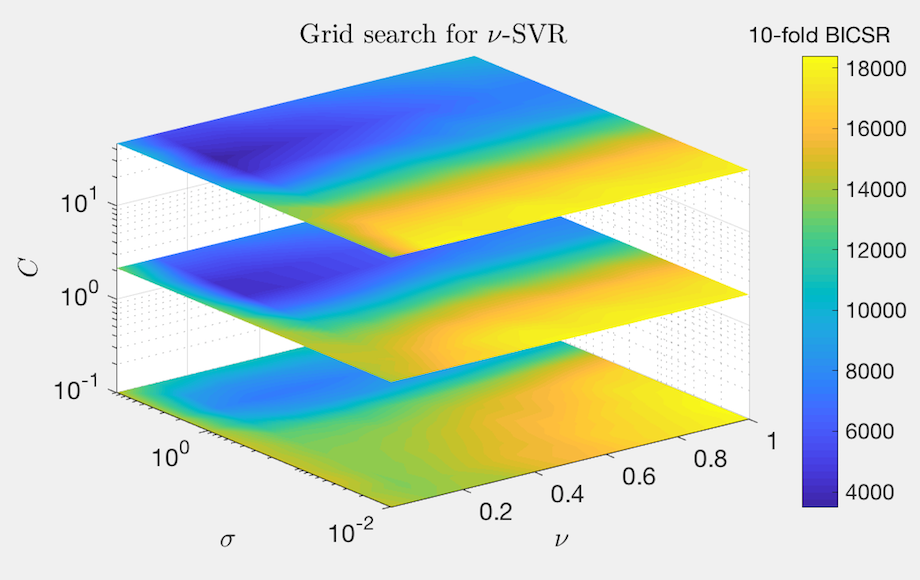
\includegraphics[width=0.85\linewidth]{gridSearch_nuSVR_BIC_airfoils}
						\caption{Grid search for $\nu$-SVR over $\nu$, $C$ and $\sigma$ for airfoils dataset \\ Best hyperparameters: $\nu = 0.11$, $C = 46.4$, $\sigma = 2.15$}
						\label{fig::gridSearch_BIC_nuSVR_airfoils}
					\end{center}
				\end{figure}
				
				\noindent Figures (\ref{fig::gridSearch_BIC_epsSVR_airfoils}) and (\ref{fig::gridSearch_BIC_nuSVR_airfoils}) expose obtained results for both $nu$-SVR and $\epsilon$-SVR. General behavior of the algorithms to the different hyperparameters variations seemed consistent with observations made on the artificial sinc dataset.  Again, distinct wells could be observed when displaying the objective function evolution leading to the conclusion that  found optimums are global. For $\epsilon$-SVR, the optimal hyperparameters values lead to a Mean Square Error of 0.185 for 295 support vectors while $\nu$-SVR yields 249 support vectors for a MSE of 0.20.
				
				  \begin{figure}
					\begin{center}
						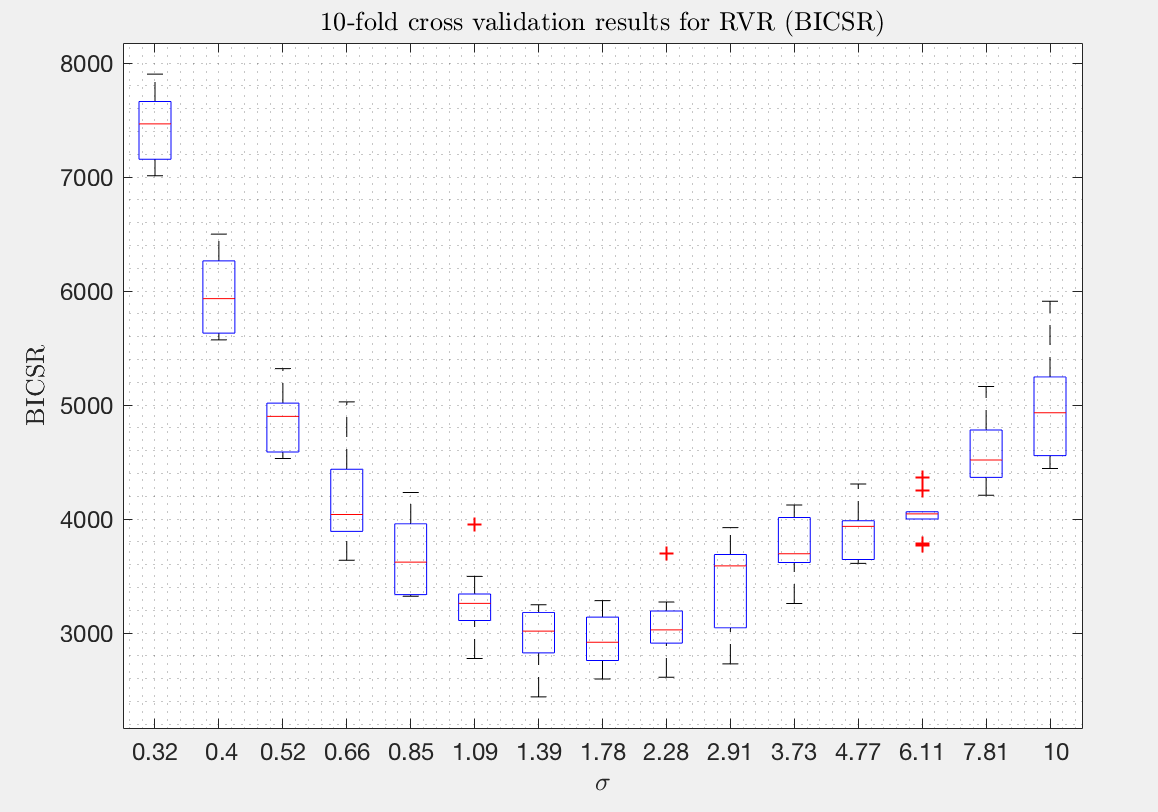
\includegraphics[width=0.8\linewidth]{airfoils_gridsearch_RVR_BIC}
						\caption{Grid search for RVR  over $\sigma$ for airfoils dataset. Best hyperparameter: $\sigma = 1.78$}
						\label{fig::airfoils_gridsearch_RVR_BIC}
					\end{center}
				\end{figure}
				

				\noindent Results of grid search over $\sigma$, the kernel width for Relevance Vectors Regression are displayed on figure (\ref{fig::airfoils_gridsearch_RVR_BIC}). Optimal kernel width therefore corresponds to $\sigma = 1.78$ leading to an MSE of 0.20. Number of retrieved relevance vectors is 66. Again, for this real dataset,  the RVR optimum leads to equivalent generalization performance but with a lot more sparsity.
				

				
				
				
			}
			
		}
	}
	\section{Discussion}
	{
		\label{section::discussion}
		\subsection{The BICSR metric}
		{
			The use of the hand-designed BICSR metric deserves some further justification. As a reminder, the BICSR writes : 
			\begin{equation}
				BICSR = N\frac{MSE}{\sigma^2} + kln(N)
			\end{equation}
			with $N$ the number of datapoints, $MSE$ the mean-squared error on the dataset, $\sigma^2$ the dataset's noise variance and $k$ the number of support vectors. 
			\subsubsection{Model likelihood estimation}
			{
				When applied to an artificial dataset, the noise variance $\sigma^2$ is known. However, this parameter must be estimated for any arbitrary dataset. Hence, in order to find, for a given model, its related optimal hyper-parameter (with respect to the BICSR), we first need, equivalently, to estimate the noise precision coefficient $\beta = \frac{1}{\sigma^2}$. \newline
				The RVR already provides a rather robust estimate of $\beta$, without bootstrapping from any initial value (automatic relevance determination), and without need for much parameters tuning. We therefore suggest the following approach for determining $\beta$ : 
				\begin{enumerate}
					\item Run a cross-validation for the RVR with a the MSE metric on the dataset
					\item Identify the optimal kernel-width (or equivalently any given kernel hyperparameter)
					\item Set $\sigma = \frac{1}{\sqrt{\beta}}$ with $\beta$ the precision given by the RVR with the previously defined kernel width
				\end{enumerate}
				To justify the use of this method, we applied it on our artificial dataset, and measured an empirical noise variance $\sigma^2 = 0.008$ instead of $0.01$. 
			}
			
			\subsubsection{BICSR validation}
			{
				To further justify this approach, we wanted to evaluate the tradeoff found by the BICSR. To do this, we cross-validate (10 folds, 0.75 training-test ratio) several $\nu$-SVR arbitrary models (hence with arbitrary hyperparameters - kernel width, $\nu$ and $C$) and plot them on a MSE versus fraction of support vectors figure. We repeated this experiment with the models generated by the optimal BICSR and MSE metrics. As shown in (\ref{fig::bicsr_valid}), the BICSR optimal model can be found at the elbow of the MSE vs sparsity curve. 
				\begin{figure}[h!]
					\begin{center}
						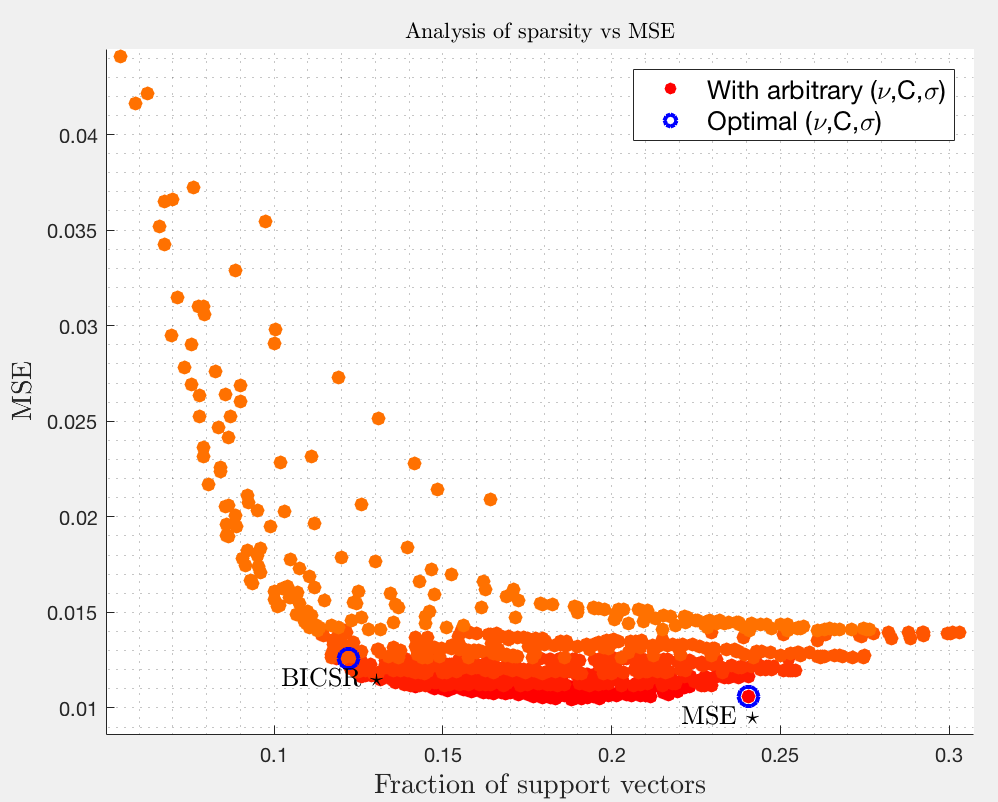
\includegraphics[width=0.85\linewidth]{bic_lnN_eval}
						\caption{BICSR and MSE optimal models evaluation}
						\label{fig::bicsr_valid}
					\end{center}
				\end{figure}
				\newline As previously introduced, the BICSR metric measures the tradeoff between MSE and sparsity. It linearly penalizes the number of support vectors, proportionally to $ln N$. We wondered if some other (utlimately better, depending on the end goal) tradeoff could be found by changing the nature of this penalization. For instance, we could think of a non-linear penalization of the numbers of support vectors (a quadratic penalization would lead to sparser models, and a logarithmic one to more accurate ones). Figure (\ref{fig::bicsr_penal}) displays the MSE versus sparsity models found when varying the nature of the penalization. Hence, it seems that our initial metric (designated as BISCR) naturally finds a rather interesting tradeoff for generalization against sparsity.  We will therefore use it as our baseline metric for the different model comparaisons. 
				\begin{figure}[h!]
					\begin{center}
						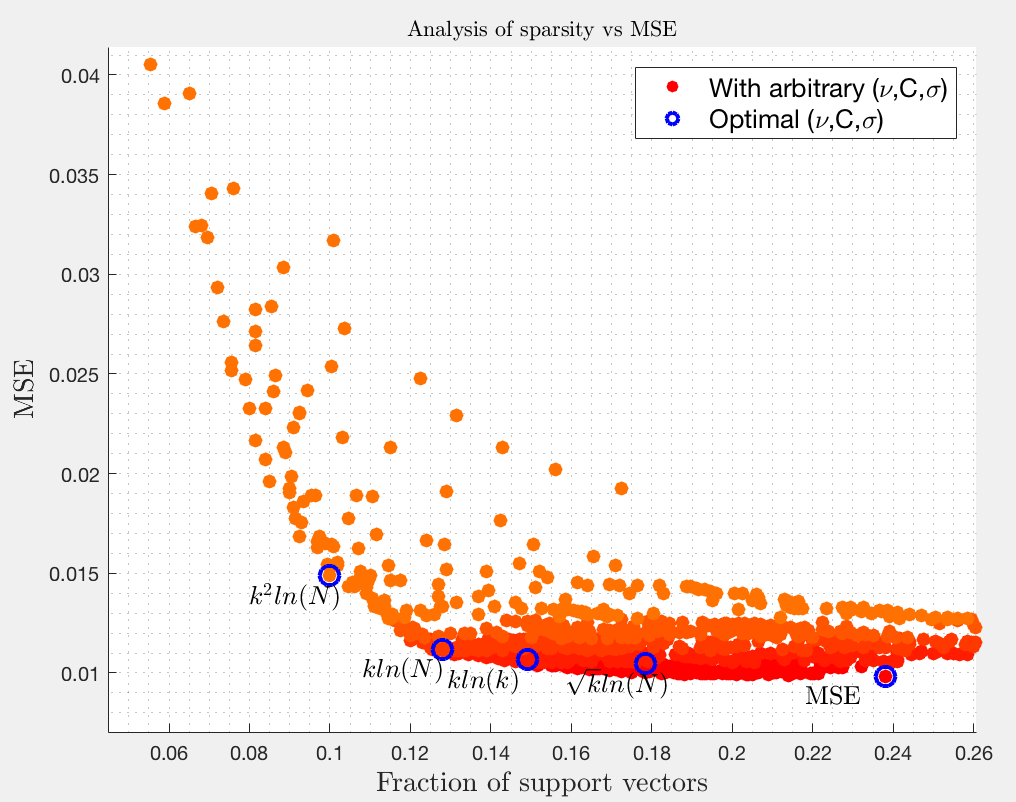
\includegraphics[width=0.85\linewidth]{bic_penal_eval}
						\caption{Evaluation for different penalizing terms}
						\label{fig::bicsr_penal}
					\end{center}
				\end{figure}
				
			}
			\subsubsection{Model comparaison}
			{
				Now that we have more insights into how our metrics behave, it is possible to compare the different models that maximize it. 
				
				\begin{figure}
					\begin{center}
						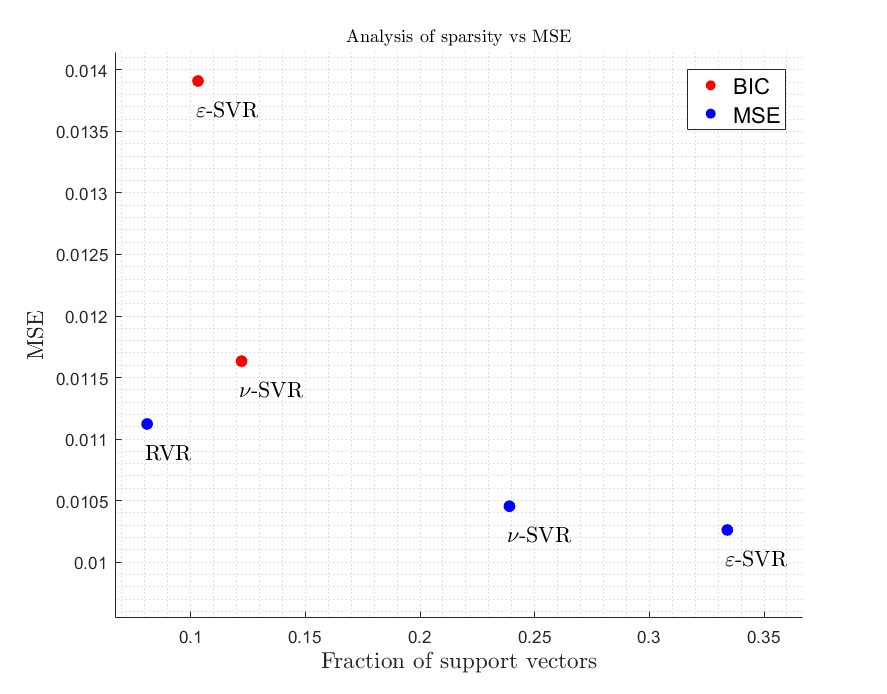
\includegraphics[width=0.75\linewidth]{ROC_sinc}
						\caption{Evaluation of the tradeoff between raw performance ($MSE$) and for each method and each metric for the sinc dataset.}
						\label{fig::ROC_sinc}
					\end{center}
				\end{figure}
				
				Figure~\ref{fig::ROC_sinc} allows us to see how the different methods react to the trade-off sparsity versus performance (which is measured by MSE minimization).
				
				First of all, we see that except from the $\varepsilon$-SVR maximizing the BICSR, all MSE values are comparable (around $15\%$ difference). However, there is a big gap in terms of sparsity since SVR with the MSE metrics have about twice as much support vectors as SVR that minimizes the BICSR metric.
				
				The key insights from this figure are that SVR methods with MSE objective have many support vectors, and that the BICSR metric leads to sparser solutions with minimal increase of the MSE. RVR achieves the best sparsity by far with minimal MSE increase and there is almost no difference between the models selected by the two different metrics.
				
				\begin{figure}
					\begin{center}
						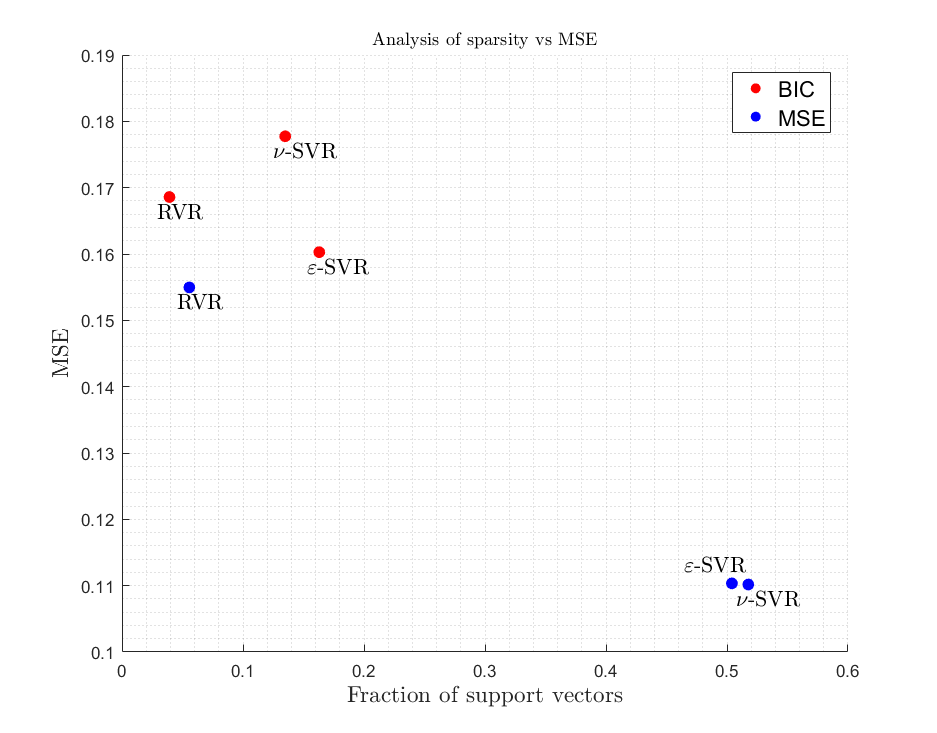
\includegraphics[width=0.75\linewidth]{airfoils_sparsity_MSE}
						\caption{Evaluation of the tradeoff between raw performance ($MSE$) and for each method and each metric for the airfoils dataset.}
						\label{fig::ROC_airfoils}
					\end{center}
				\end{figure}
			
				The sinc dataset was a bit too easy for our methods, which is why MSE values were close. Figure \ref{fig::ROC_airfoils} shows the same curve as before but for the airfoils dataset. We can observe now that the difference in terms of MSE is significant (up to $70\%$). The difference in sparsity is also huge since $SVR$ solutions minimizing the MSE have 10 times more support vectors than RVR solutions (50\% of the dataset versus 5\%). We see that $\nu$-SVR and $\varepsilon$-SVR perform relatively similarly (although there is a little difference for the BICSR metric), and that they are very sensitive to the change of metric. On the other hand, RVR solutions are close to solutions for SVR using the BICSR metric. Again, RVR is not very sensitive to the metric used although there is now a difference between the two.
				
				\newline To summarize, RVR should be prefered when sparsity is a key feature because it always leads to sparser solutions than SVR (with better MSE for comparable levels of sparsity) and is less sensitive to the choice of the metric. On the other hand, this insensivity may be a problem since it only leads to very sparse solutions. To find the best MSE while staying under a relatively high given threshold of support vectors (0.3 for example) then it is possible to tweak a metric (BICSR with sublinear penalization on the number of support vectors for example) and then to use SVR, whereas RVR would almost always give the same result.
				
				Not that here we use the same set for cross-validation and testing. This may lead the hyper-parameters to overfit the cross-validation set, therefore leading to lower scores than one would expect at generalization. However, this is not critical for our study since we are more interested in the impact of the metrics and not the true generalization of our methods.
			}
		}
		\subsection{Behavior far from data}
		{
			If we focussed until now on the tradeoff between sparsity and generalization performances, their are other aspects worthy of discussion. Namely, the two considered methods (SVR and RVR) could be compared on the basis of \emph{generalization far from the data}. 
			\newline On this particular question, both methods show the same drawbacks. Indeed, the predicted function far from data is limited to the learned bias (at least for centered kernels, like the Gaussian RBF). One could argue that this drawback is limited for the RVR, as the variance of the predictive distribution should grow as we get far from the data, indicating that predictions are not to be trusted with. However, (\ref{eq::predictive}) proves that this assumption does not hold, as for the RVR the predictive distribution is higher close from the data, and constant far from it. 
			\newline Therefore, both methods are not to be trusted with far from the data (they only capture the regressive function's mean and not the general trend). Other Bayesian methods, like Gaussian Process Regression would probably do a better job at this particular task - but use the entire dataset when making predictions. 
		}
	}
	\section{Conclusion}
	{

	}
	
	% \newline RVR lies in the family of bayesian methods for regression, it is therefore possible to derive a likelihood expression as in equation (\ref{eq::rvr_likelihood}). In this case, the log-likelihood of the model therefore writes:. Even though no likelihood expression can be derived for SVR, analogies between both methods lead to use previous equation to design the sparse regression evaluative metric in case of SVR.  

			\begin{equation}
			ln(L(\mathbf{t}{,X,w,\beta})) =  -\frac{1}{2}\beta^2 \sum_{i=1}{N}(t_n - y(x_n))^2
			\end{equation}
			where we recall that estimated parameter $\beta$ is supposed to represent the precision (inverse of the variance) of the noise affecting the output. Therefore, a
	
	\bibliographystyle{plain}
 	 \bibliography{bib_file}
	
\end{document}